\documentclass{prettytex/ox/mmsc-special-topic}
\usepackage{tabularray}
\usepackage{pdfpages}
\setlength{\headheight}{19.53pt}

\setcounter{biburllcpenalty}{7000}
\setcounter{biburlucpenalty}{8000}

\addbibresource{sources.bib}
\tikzexternalize[prefix=tikz/]

\newcommand{\topictitle}{
  Melon - a Task Scheduling Package for Personal Todo Lists \\
  \normalsize using Markov Chain Monte-Carlo Methods
}
\newcommand{\candidatenumber}{1072462}
\newcommand{\course}{Python in Scientific Computing}

\title{\topictitle}
\author{Candidate \candidatenumber}
\date{\today}

\makenoidxglossaries
\newacronym{ode}{ODE}{Ordinary Differential Equation}
\newacronym{pde}{PDE}{Partial Differential Equation}
\newacronym{gui}{GUI}{Graphical User Interface}

\begin{document}
  \pagestyle{plain}
  \mmscSpecialHeader

  \begin{abstract}
    \label{abstract}
    In this project report we will review the central concepts utilised in the group work conducted to make progress in the \gls{pde} problem associated with the electrochemical model of a battery cell and present numerical results.
    \vspace*{0.2cm}

    \noindent
    \textbf{Our Goal:}
    Numerically obtain the solution $\{a(x, T), b(x, T)\}$.

    The Finite Difference schemes are implemented in Julia and Python, whereas the Spectral Method is implemented in C++.
  \end{abstract}

  \begin{figure}[H]
    \centering
    % \includegraphics[width=\linewidth]{figures/screenshot.png}
    \caption{The \gls{gui} of the Spectral Solver.}
    \label{fig:gui}
  \end{figure}

  \pagebreak
  \pagestyle{normal}

  \section{Problem Introduction}
  \label{sec:introduction}

  UIDs are useful because they make collisions very unlikely, which is not to say that these should not be checked, but if two clients are connected that each generated a set of UIDs it is very unlikely to have to do conflict resolving.

  We recommend usage with \texttt{xandikos}, a version-controlled DAV server, capable of syncing calendars (events, todos and journals) and contacts.

  Published on PyPi.

  \subsection{Usage}
  % TODO: describe installation, etc., running main.py
  Use \texttt{invoke -l} to list all available tasks.

  Is platform-independent, for example due to the usage of \texttt{pathlib.Path}.

  \section{Underlying Theory}
  \begin{algorithm}[language=pseudo,caption={\centering The Metropolis-Hastings algorithm \parencite{metropolis, hastings}},basicstyle=\footnotesize]
until convergence, repeat
  sample a candidate $\vec{x}^*$.
  set $\vec{x}^{n+1} = \vec{x}^*$ with acceptance probability
    $p_{\rm accept} = \min\left(1, \e^{-\beta (F^{n+1} - F^n)}\right)\,,$ with $\beta \in \R^+$ a transition factor.
  Otherwise, let $\vec{x}^{n+1} = \vec{x}^{n}$.
  \end{algorithm}

  \section{Code Quality}
  \subsection{Formatting}
  \subsection{Docstrings}
  \subsection{Documentation}
  \subsection{Tests}
  Server can be started using Docker.

  \subsubsection{Coverage}
  \subsection{Type Checking}
  Using \texttt{pyright} instead of \texttt{mypy} as it is much faster.
  \subsection{Using Appropriate Language Features}
  Using \texttt{autoflake} and \texttt{pyupgrade}.
  Used \texttt{logging}.
  \subsection{Maintaining Code Quality}
  Using \texttt{pre-commit} and GitHub Actions CI/CD.
  Uses \texttt{invoke} to manage common development tasks.

  \begin{minted}{python}
    import numpy
    x = 5
    print(x ** 2)
  \end{minted}

  interrogate -v einfügen

  \begin{table}[H]
    \centering
    \caption{RESULT: PASSED (minimum: 80.0\%, actual: 100.0\%)}
    \begin{tabular}{lllll}
      \hline
      \bf Name                        & \bf Total & \bf Miss & \bf Cover & \bf Cover \\
      \hline
      main.py                         & 2         & 0        & 2         & 100\%     \\
      tasks.py                        & 8         & 0        & 8         & 100\%     \\
      docs/conf.py                    & 1         & 0        & 1         & 100\%     \\
      melon/\_\_init\_\_.py           & 1         & 0        & 1         & 100\%     \\
      melon/calendar.py               & 11        & 0        & 11        & 100\%     \\
      melon/config.py                 & 1         & 0        & 1         & 100\%     \\
      melon/melon.py                  & 19        & 0        & 19        & 100\%     \\
      melon/todo.py                   & 20        & 0        & 20        & 100\%     \\
      melon/visualise.py              & 3         & 0        & 3         & 100\%     \\
      melon/scheduler/\_\_init\_\_.py & 1         & 0        & 1         & 100\%     \\
      melon/scheduler/base.py         & 10        & 0        & 10        & 100\%     \\
      melon/scheduler/cpp.py          & 3         & 0        & 3         & 100\%     \\
      melon/scheduler/numba.py        & 8         & 0        & 8         & 100\%     \\
      melon/scheduler/purepython.py   & 12        & 0        & 12        & 100\%     \\
      melon/scheduler/rust.py         & 3         & 0        & 3         & 100\%     \\
      melongui/\_\_init\_\_.py        & 1         & 0        & 1         & 100\%     \\
      melongui/calendarlist.py        & 6         & 0        & 6         & 100\%     \\
      melongui/mainwindow.py          & 14        & 0        & 14        & 100\%     \\
      melongui/taskitemdelegate.py    & 12        & 0        & 12        & 100\%     \\
      melongui/tasklist.py            & 14        & 0        & 14        & 100\%     \\
      melongui/taskwidgets.py         & 8         & 0        & 8         & 100\%     \\
      tests/\_\_init\_\_.py           & 1         & 0        & 1         & 100\%     \\
      tests/test\_melon.py            & 7         & 0        & 7         & 100\%     \\
      tests/test\_scheduler.py        & 9         & 0        & 9         & 100\%     \\
      \hline
      \bf TOTAL                       & 175       & 0        & 175       & 100.0\%   \\
      \hline
    \end{tabular}
  \end{table}

  Screenshot von gnome-calendar

  Screenshot GUI

  \subsection{Autocorrelation Analysis}
  \subsection{Coole Pie-Plots mit Verteilungen}

  \section{Runtime Performance}
  \begin{minted}{python}
In [1]: %timeit str(t.icalendar_component["uid"])
  122 µs ± 1.06 µs per loop (7 runs, 10,000 loops each)
In [2]: %timeit t.vtodo.contents["uid"][0].value
  355 ns ± 7.14 ns per loop (7 runs, 1,000,000 loops each)
In [3]: %timeit t.vobject_instance.contents["vtodo"][0].contents["uid"][0].value
  296 ns ± 7.06 ns per loop (7 runs, 1,000,000 loops each)
In [4]: %timeit t._vobject_instance.contents["vtodo"][0].contents["uid"][0].value
  208 ns ± 23.7 ns per loop (7 runs, 10,000,000 loops each)
  \end{minted}

  \begin{table}[H]
    \centering
    \caption{Profile obtained by running \mintinline{bash}{./main.py --profile & grep todo.py}.}
    \begin{tabular}{rrrrrll}
      \hline
      ncalls & tottime & percall & cumtime & percall & filename:lineno & function     \\
      \hline
      16958  & 0.008   & 0.000   & 0.939   & 0.000   & todo.py:36      & vtodo        \\
      32475  & 0.047   & 0.000   & 0.705   & 0.000   & todo.py:96      & uid          \\
      856    & 0.003   & 0.000   & 0.579   & 0.001   & todo.py:26      & upgrade      \\
      117    & 0.000   & 0.000   & 0.489   & 0.004   & todo.py:111     & priority     \\
      417    & 0.001   & 0.000   & 0.461   & 0.001   & todo.py:121     & isIncomplete \\
      5512   & 0.003   & 0.000   & 0.278   & 0.000   & todo.py:45      & summary      \\
      856    & 0.002   & 0.000   & 0.112   & 0.000   & todo.py:21      & \_\_init\_\_ \\
      1363   & 0.006   & 0.000   & 0.024   & 0.000   & todo.py:164     & \_\_lt\_\_   \\
      7844   & 0.004   & 0.000   & 0.009   & 0.000   & todo.py:61      & dueDate      \\
      2605   & 0.001   & 0.000   & 0.003   & 0.000   & todo.py:85      & dueTime      \\
    \end{tabular}
  \end{table}

  \begin{table}[H]
    \centering
    \caption{Profile obtained by running \mintinline{bash}{inv profile-scheduler & grep purepython.py}.}
    \begin{tabular}{rrrrrll}
      \hline
      ncalls  & tottime & percall & cumtime & percall & filename:lineno   & function         \\
      \hline
      1       & 0.000   & 0.000   & 14.236  & 14.236  & purepython.py:142 & schedule         \\
      10      & 0.209   & 0.021   & 14.235  & 1.424   & purepython.py:123 & mcmcSweep        \\
      36010   & 1.144   & 0.000   & 13.784  & 0.000   & purepython.py:97  & computeEnergy    \\
      2196671 & 5.391   & 0.000   & 11.353  & 0.000   & purepython.py:41  & spreadTasks      \\
      1006332 & 1.389   & 0.000   & 1.842   & 0.000   & purepython.py:27  & generateNextSlot \\
      2196610 & 0.798   & 0.000   & 0.972   & 0.000   & purepython.py:108 & <genexpr>        \\
      2196610 & 0.384   & 0.000   & 0.384   & 0.000   & purepython.py:106 & <genexpr>        \\
      36000   & 0.082   & 0.000   & 0.217   & 0.000   & purepython.py:83  & permuteState     \\
      36011   & 0.046   & 0.000   & 0.124   & 0.000   & purepython.py:19  & startingSlot     \\
      % 61      & 0.000 & 0.000 & 0.000  & 0.000  & purepython.py:152 & <genexpr>
      % 1       & 0.000 & 0.000 & 0.000  & 0.000  & purepython.py:71  & __init__
      % 1       & 0.000 & 0.000 & 0.000  & 0.000  & purepython.py:14  & __init__
    \end{tabular}
  \end{table}

  \section{Results}
  \begin{figure}[H]
    \centering
    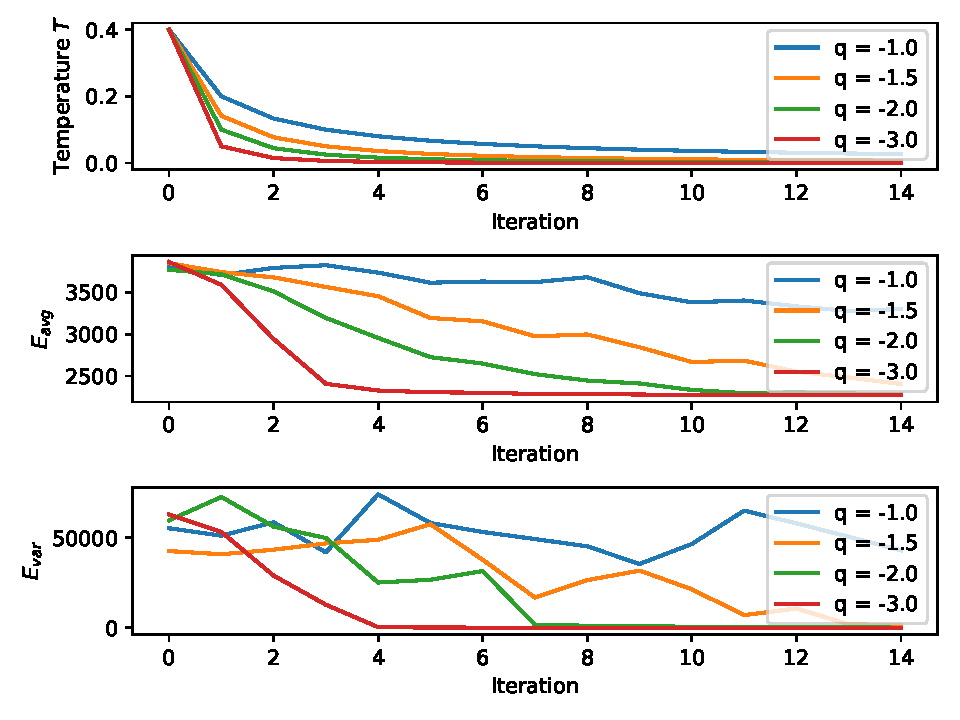
\includegraphics[width=0.8\linewidth]{results/convergence.pdf}
    \caption{Convergence}
  \end{figure}

  Numba Compilation time: 2.5625428539933637

  \begin{table}[H]
    \vspace{0.5cm}
    \centering
    \caption{Runtime Comparison of the different implementations run on the same scenarios. Each runtime is given as the average over three runs. The finite difference schemes (for the one-dimensional case) were run with $N_x = N_t = 4000$ up to $T = 40$. The spectral method was run using a series expansion of order 15, also up to $T = 40$. The remaining parameters ($\alpha$, $\kappa_0$, $E_0$, etc.) were all identical.}
    \begin{tblr}{
      colspec={llr},
      row{2,3} = {bg=azure9},
          row{4} = {bg=violet9},
          row{5} = {bg=cyan9},
        }
      \hline
      \bf Implementation & \bf Language & \bf Runtime / seconds \\
      \hline
      MCMCScheduler      & Python & 16.6180 \\
      NumbaMCMCScheduler & Python & 1.3117 \\
      \hline
      RustyMCMCScheduler & Rust & 0.3660 \\
      \hline
      CppMCMCScheduler   & C++ & 0.1513
      \hline
    \end{tblr}
    \label{table:runtime}
  \end{table}


  \section{Acknowledgements}
  The visualisation code (\texttt{visualise.py}) is adapted from \cite{monte-carlo-todo-lists}.

  The task check icon is the logo of the \textit{Tasks.org} Free and Open Source Android App, which may be found \href{https://github.com/tasks/tasks/tree/main/graphics}{here}.

  \pagebreak
  \printbibliography
  \printnoidxglossary[type=acronym]

  \appendix
  \includepdf[pages=7-29]{../build/docs/latex/melon.pdf}
\end{document}
